\documentclass[10pt]{article}
\usepackage[letterpaper,margin=1in]{geometry}
\usepackage{lmodern}
\usepackage[T1]{fontenc}
\usepackage[utf8]{inputenc}
\usepackage{amsmath,amssymb}
\usepackage{graphicx}
\usepackage{booktabs}
\usepackage{tabularx}
\usepackage{enumitem}
\usepackage[font=small,labelfont=bf]{caption}
\usepackage[hidelinks]{hyperref}
\usepackage{microtype}

\setlist{itemsep=2pt,topsep=4pt}
\renewcommand{\topfraction}{0.9}\renewcommand{\bottomfraction}{0.8}\renewcommand{\textfraction}{0.07}\renewcommand{\floatpagefraction}{0.75}
\graphicspath{{fig/}}
\newcommand{\Fh}{F_{0.5}}
\newcommand{\N}{\mathcal{N}}

\title{\textbf{Business Entity Resolution at Scale:\\ Reverse-Engineering a Corruption Process\\ to Match 11.7 Million Records}}
\author{Team Grokking: Divyanshu (team leader), Aaditya Rawat, Shristi Chandra\\[2pt]
\small\itshape Amazon ML Challenge 2026 --- Business Entity Resolution\\
\small September 2026 \quad$\cdot$\quad Code: \texttt{er/} \quad$\cdot$\quad Log: \texttt{experiments/experiments.csv}}
\date{}

\begin{document}
\maketitle

\begin{abstract}
\noindent Three independent sources describe the same businesses with different, deliberately corrupted names and addresses, and share no identifiers. For each record of the clean reference source S1, the task is to find every record in the noisy sources S2 and S3 that refers to the same business. Scoring is macro $\Fh$ per S1 entity, which weights precision twice as heavily as recall and counts every entity with no true match. We treat the problem as \emph{inverting a data-generating process}. Forensic analysis of 12.5M training records showed a small set of corruption operators and a population of adversarial \emph{near-miss decoys}: copies of real businesses with the house number shifted. The system retrieves candidates with typed-token TF-IDF and exact structured keys, scores pairs with a two-stage gradient-boosted model whose second stage reasons over whole entities, and assigns every record to at most one business. Every component was admitted by a pre-registered ablation rule. On 1.94M training entities never used for training, processed exactly as the test set is, the system reaches macro $\Fh = 0.961$ (US 0.971, India 0.947), up from 0.640 for a rules baseline; on held-out states it reaches 0.973. The submitted configuration prunes the candidate set by rule to 22 candidates per S1 on the test set (3$\times$ fewer) at a held-out cost of 0.0017 ($\Fh = 0.971$).
\end{abstract}

\noindent\textbf{Keywords:} entity resolution; record linkage; blocking; learning to match; gradient boosting; macro $\Fh$; data forensics; transliteration.

\section{Introduction}

Entity resolution decides which records, drawn from sources that share no key, describe the same real-world object. The version studied here has three sources of business records, each with only a name, an address and a country label. Source~1 is clean and deduplicated; sources~2 and~3 contain zero or more noisy copies of each S1 business, plus unrelated distractors. The training set has 2.21M S1, 5.03M S2 and 5.29M S3 records with ground truth; the test set has 1.73M S1 and 9.97M S2/S3 records and adds a third country, France, that never appears in training.

The standard recipe---normalise strings, block on keys, score pairs with fuzzy-match features, threshold---is a reasonable starting point but leaves most of the available signal unused here. The data is synthetic, generated by a corruption process that treats true copies and decoys differently. Measuring that process first, and designing features that model it directly, is worth far more than extra model capacity: comparing the full set of house numbers instead of the first one raised the score by 0.197 on its own (Section~\ref{sec:ablation}).

\subsection{Contributions}
\begin{itemize}
\item A quantitative reconstruction of the data-generating process, including the near-miss decoy population and the finding that addresses are corrupted once per source while names are corrupted per record (Section~\ref{sec:forensics}).
\item A retrieval stage combining typed-token TF-IDF with exact structured keys, which retrieves 97.1\% of true pairs at 46 candidates per S1 (Section~\ref{sec:retrieval}).
\item A two-stage matcher whose second stage uses entity-level evidence: competing S1s, siblings sharing a corrupted address, and support from the other source (Section~\ref{sec:model}).
\item A scale-consistent inference scheme (state blocks) and a validation design by whole states that keeps decoys in the same split as the entities they imitate (Sections~\ref{sec:arch} and~\ref{sec:method}).
\item An analytic acceptance condition for macro $\Fh$ (eq.~\ref{eq:marginal}) that explains why a single global threshold is near-optimal, and an error anatomy showing that the remaining loss is retrieval-bound, not scorer-bound (Section~\ref{sec:anatomy}).
\item A complete, honest ablation record, including the components that were tested and rejected (Appendix~\ref{app:log}).
\end{itemize}

\section{Problem and Metric}
For an S1 entity $e$ with true match set $M_e$ and predicted set $\hat M_e$,
\begin{equation}
\Fh(e) = \frac{(1+\beta^2)\,P_e R_e}{\beta^2 P_e + R_e} = \frac{1.25\,|\hat M_e \cap M_e|}{0.25\,|M_e| + |\hat M_e|}, \qquad \beta = 0.5,
\label{eq:f05}
\end{equation}
\begin{equation}
\text{Score} = \frac{1}{|S_1|}\sum_{e\in S_1} \Fh(e), \qquad \Fh(e) = 1 \text{ if } M_e = \hat M_e = \emptyset.
\label{eq:macro}
\end{equation}
Two properties shape every design decision. With $\beta = 0.5$ a false merge costs roughly twice as much as a missed link, so an uncertain record should usually be left unassigned. The average is over entities, not pairs, and \emph{singletons count}: an S1 with no true matches scores 1 for an empty prediction and 0 for any prediction. With 5.6\% singletons, one wrong merge on each would cost 0.056 by itself.

\paragraph{Worked example.} For the README case, predicted $\{$S2-00047, S2-00193, S3-00812$\}$ against truth $\{$S2-00047, S3-00812$\}$: $|\hat M \cap M| = 2$, $|M| = 2$, $|\hat M| = 3$, so $P = 2/3$, $R = 1$ and $\Fh = 1.25\cdot 2/(0.25\cdot 2 + 3) = 2.5/3.5 = 0.714$. Our metric implementation reproduces this value in a self-test run before every experiment.

\section{Data Forensics: Reconstructing the Generator}
\label{sec:forensics}
Before choosing a model we measured what the generator does. Each claim was checked on the full training files or on a stratified sample of 67k S1 entities with all their matches (Table~\ref{tab:facts}).

\begin{table}[htbp]
\centering\small
\caption{Verified structural facts and their design consequences.}
\label{tab:facts}
\begin{tabularx}{\linewidth}{@{}p{3.6cm}Xp{3.9cm}@{}}
\toprule
Finding & Measurement & Consequence \\
\midrule
One owner per record & 0 violations in 7.64M labels & assign each record to at most one S1 \\
Matches per S1 & 0--11, mode 3; 5.6\% singletons & singletons dominate precision risk \\
Distractors & 27\% of S2/S3 match nothing (1.34M per source) & candidates must be rejectable \\
Near-miss decoys & 35--45\% of distractors: same name, city, street; shifted number & house-number relation is core \\
Country agreement & 100\% of 11,560 sampled pairs & partition by country \\
No shared Latin name token & 24\% of India, 8\% of US positives & address-only path required \\
Indic scripts & 9 scripts, token-aligned (551k pairs, 10 misaligned) & learn a token dictionary \\
Empty addresses & 3--5\% of records; 97.7\% are true matches & do not abstain on empty address \\
Postal codes & 6-digit PIN essentially never present & no postal blocking key \\
Leakage & IDs, row and label order: correlation $-0.0004$ & no identifier features \\
\bottomrule
\end{tabularx}
\end{table}

\paragraph{Two levels of corruption.} Addresses are corrupted \emph{once per source}: when two records of the same S1 from the same source both disagree with the S1 house number, they agree with each other in 92--98\% of cases, and within-source siblings are more alike (address Jaccard 0.72--0.82) than each is to S1 (0.50--0.81). Names are corrupted \emph{per record}: insertion/deletion typos (25\% of changed tokens), substitutions (15\%), leet digits (7\%), legal-form changes, token reordering, noise prefixes, ID tags, domain forms, \emph{formerly known as}/\emph{DBA} wrappers and full rebrands to random strings (2.7\%).

Table~\ref{tab:ops} gives the measured rate of each operator by source and country on 231k sampled true pairs. The rates differ enough between S2 and S3 that the source label is itself informative, and enough between countries that any fixed normalisation rule must be validated per country.

\begin{table}[htbp]
\centering\small
\caption{Corruption-operator rates on true matches (share of pairs; 231,209 sampled pairs). ``---'' = not applicable.}
\label{tab:ops}
\begin{tabular}{@{}lrrrr@{}}
\toprule
Operator & S2 US & S2 India & S3 US & S3 India \\
\midrule
Name tokens identical to S1 & 30.6\% & 17.4\% & 30.3\% & 20.1\% \\
Name tokens dropped & 17.3\% & 35.5\% & 16.2\% & 26.3\% \\
Name tokens added & 11.9\% & 6.9\% & 15.2\% & 10.0\% \\
Name tokens reordered & 6.1\% & 5.1\% & 5.9\% & 5.0\% \\
No name token shared with S1 & 7.8\% & 5.9\% & 7.8\% & 8.4\% \\
Name in Indic script & --- & 23.3\% & --- & 13.0\% \\
Accent injected into Latin name & 7.3\% & 5.1\% & 7.4\% & 6.0\% \\
Name entirely upper-case & 23.6\% & 16.3\% & 3.3\% & 2.9\% \\
Domain / handle form & 5.6\% & 4.4\% & 5.4\% & 4.7\% \\
\emph{formerly} / DBA / t/a wrapper & 0.0\% & 0.0\% & 2.4\% & 1.6\% \\
Address empty & 4.9\% & 3.9\% & 4.6\% & 4.1\% \\
Address tokens identical to S1 & 13.3\% & 11.3\% & 4.5\% & 4.3\% \\
Address components dropped & 13.7\% & 51.3\% & 2.2\% & 35.5\% \\
Address components reordered & 0.4\% & 4.9\% & 4.6\% & 30.7\% \\
House number identical & 64.6\% & 60.0\% & 66.2\% & 60.2\% \\
US state as code / full name & 94.5 / 0.6\% & --- & 6.4 / 89.1\% & --- \\
India state as 2-letter code / native script & --- & 0.0 / 20.5\% & --- & 55.2 / 18.4\% \\
\bottomrule
\end{tabular}
\end{table}

\paragraph{The decoy signature.} True matches almost always keep the S1 house number or reformat it; near-miss decoys keep name, city and street but move the number by a small amount (Figure~\ref{fig:house}). In the US, $|\Delta| \le 10$ occurs in 63.7\% of decoys and in 1.4\% of true matches. Source signatures also differ measurably (Table~\ref{tab:sources}), which is why the model receives the source as a feature.

\begin{figure}[htbp]
\centering
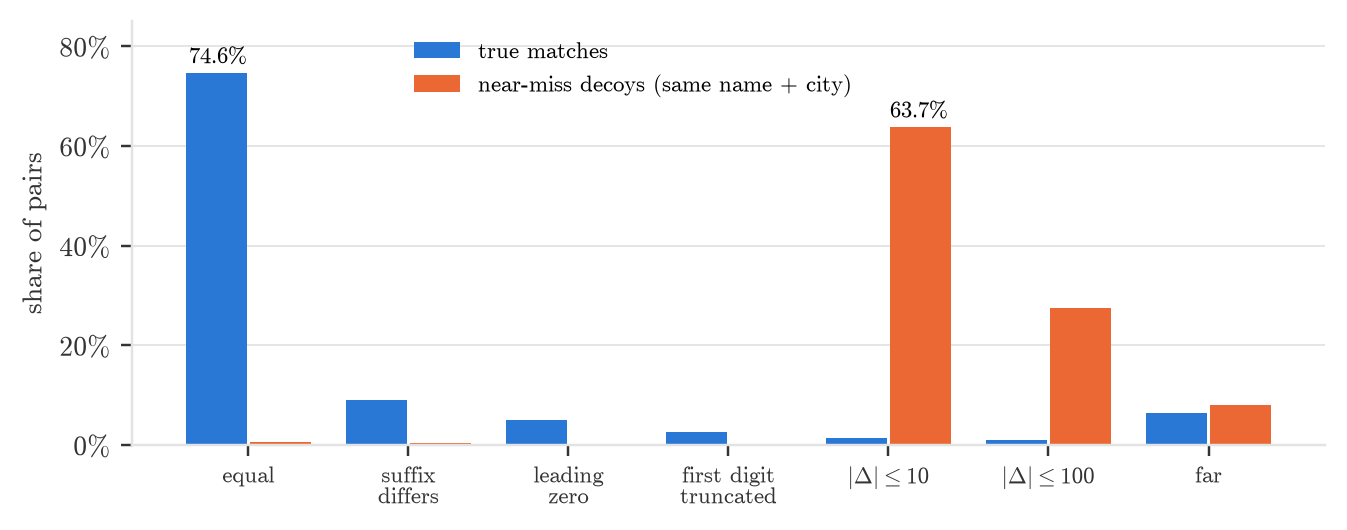
\includegraphics[width=\linewidth]{house.png}
\caption{House-number relation for true matches and near-miss decoys (US, source 2). Decoys are the same business name in the same city with the number shifted.}
\label{fig:house}
\end{figure}

\begin{table}[htbp]
\centering\small
\caption{Source-specific corruption rates (sampled positives).}
\label{tab:sources}
\begin{tabular}{@{}lcc@{}}
\toprule
Signature & Source 2 & Source 3 \\
\midrule
Name entirely upper-case & 16--24\% & 3\% \\
US state as code / full name & 94.5\% / 0.6\% & 6.4\% / 89.1\% \\
India: components dropped / reordered & 51\% / 5\% & 36\% / 31\% \\
India: name in native script & 23\% & 13\% \\
\emph{formerly} / DBA / t/a wrappers & 0\% & 1.6--2.4\% \\
US house number identical to S1 & 74.6\% & 76.1\% \\
\bottomrule
\end{tabular}
\end{table}

\section{System Architecture}
\label{sec:arch}
The pipeline (Figure~\ref{fig:arch}) is a cascade in which each stage narrows the problem for the next. Normalised \emph{views} undo the reversible corruptions; \emph{retrieval} proposes at most eight S1 candidates per record; \emph{stage~1} scores each pair on its own; \emph{stage~2} rescores surviving pairs with evidence from other pairs; \emph{assignment} makes the final one-S1-per-record decision. Stages exchange plain Parquet tables, so any stage can be replaced for an ablation without touching the others.

\begin{figure}[htbp]
\centering
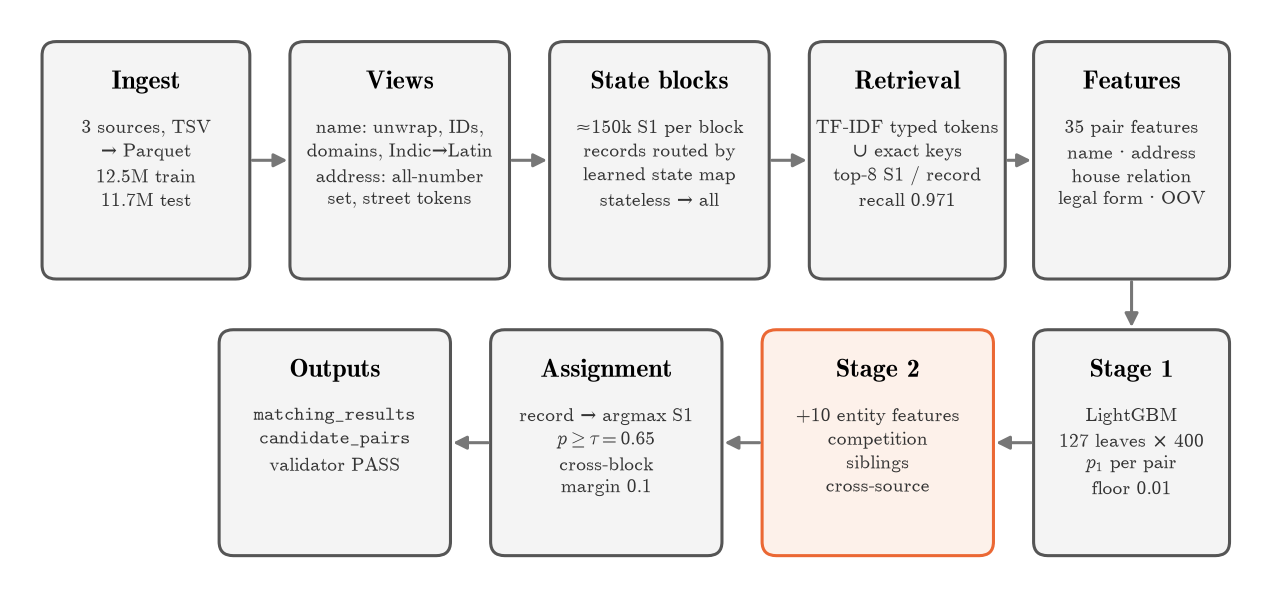
\includegraphics[width=\linewidth]{architecture.png}
\caption{System architecture. The highlighted stage is the only one that reasons over whole entities rather than single pairs.}
\label{fig:arch}
\end{figure}

\paragraph{Scale-consistent processing.} Inverse document frequencies, the posting cap, name-collision counts and the vocabulary behind the out-of-vocabulary feature all depend on how many S1 entities share a partition. The model was trained on subsets of whole states holding 76k--180k S1 per country, while a test country holds up to 810k. Full-size data is therefore processed in \emph{state blocks} of about 150k S1, so every feature takes values from the distribution it was trained on. Records are routed with a component-to-state map learned from training labels (0.04\% of true-match records misrouted); records with no recognisable state, mostly empty addresses, are scored in every block of their country.

\section{Representations}
\paragraph{Name view.} Unicode NFKD folding, accent removal and lower-casing; wrapper unwrapping, keeping the original name $Y$ in \emph{X formerly known as Y}; removal of ID tags (\texttt{\#70318}, \texttt{(ID: 96415)}) and legal forms, which are kept separately as a legal-form set $L$; segmentation of domain and handle forms (\texttt{pennington\-associates.com}) into S1-vocabulary words by a minimum-cost dynamic program (known word cost 1, unknown character cost 2); and Indic$\to$Latin transliteration with a 1,498-token dictionary learned by positionally aligning native-script names with their S1 names, which covers 96.4\% of Indic tokens in the test set.

\paragraph{Address view.} The view keeps the token set, the alphabetic street tokens and the set of all numbers $\N(\cdot)$, with leading zeros removed. Comparing only the first number fails in India, where the generator injects a random \texttt{DOOR NO} prefix, and whenever components are reordered. The comparison functions are
\begin{equation}
J(A,B) = \frac{|A\cap B|}{|A\cup B|}, \qquad \operatorname{cover}(r,e) = \frac{|\N(e)\cap\N(r)|}{|\N(e)|},
\label{eq:jacc}
\end{equation}
\begin{equation}
\Delta(r,e) = \bigl|\min(\N(e)\setminus\N(r)) - \min(\N(r)\setminus\N(e))\bigr|.
\label{eq:delta}
\end{equation}

\paragraph{Worked example.} S1 \emph{Autrey Factory Inc, 2626 Belmont Avenue, Phoenix} against decoy \emph{Co Autrey Factory, 2631 BELMONT AVENUE, PHOENIX}. After legal-form removal both names are $\{$autrey, factory$\}$ and the name Jaccard is 1.0, but $\N(e) = \{2626\}$ and $\N(r) = \{2631\}$, so cover $= 0$ and $\Delta = 5$: the decoy signature of Figure~\ref{fig:house}. A true copy written \emph{02626 BELMONT AVE} gives $\N(r) = \{2626\}$ and cover $= 1$.

\section{Candidate Generation}
\label{sec:retrieval}
Retrieval runs from record to S1: each record has at most one true S1, so keeping the top $k$ S1 per record bounds candidate volume without truncating S1s that have many copies. \textbf{R-sparse} represents each entity as a bag of typed tokens---name tokens, alphabetic address tokens, numbers, number+street and number+name pairs---so that a house number is informative only in the context of its street or name. With $N_c$ S1 entities in block $c$,
\begin{equation}
w_t = \Bigl(\log \frac{N_c}{\mathrm{df}_t}\Bigr)^2 \quad (\mathrm{df}_t \le 100), \qquad s(r,e) = \frac{\sum_{t\in T(r)\cap T(e)} w_t}{\sqrt{\sum_{t\in T(e)} w_t}}.
\label{eq:idf}
\end{equation}
For $N_c = 150{,}000$, a number+street token shared by 10 entities has $w = (\ln 15{,}000)^2 = 9.616^2 = 92.5$, and a name token with $\mathrm{df} = 100$ has $w = (\ln 1{,}500)^2 = 53.5$. Tokens with $\mathrm{df} > 100$ are dropped: a cap of 300 would triple the join volume (389 versus 131 postings per record) for no measured gain. \textbf{R-exact} adds exact keys (sorted name key, number+street, number+name), drops keys shared by more than 50 S1, and keeps the eight S1 with most shared keys per record.

\paragraph{Cost model.} The join volume of R-sparse for a record $r$ is $\sum_{t\in T(r),\,\mathrm{df}_t\le c}\mathrm{df}_t$: the sum of posting-list lengths of its tokens under the cap $c$. Measured on a 256k-entity partition this is 131 postings per record at $c=100$, 389 at $c=300$ and 1,614 at $c=1{,}000$, so the cap is the single knob that trades recall for memory; at $c=100$ a 1.2M-record partition costs $\approx$157M join rows, processed in 16 record chunks so that no chunk exceeds 5\,GB. R-exact adds a bounded $\le 50$ postings per key. The union is at most $16$ S1 per record before deduplication, and 46 records per S1 on average after it.

\paragraph{Candidate pruning.} Because smaller candidate sets are ranked higher in the final evaluation, the union is pruned by two rules that use no model: a candidate is kept only if its TF-IDF score is at least $0.5\times$ the record's best score or it has the record's most shared exact keys; then each S1 keeps its 50 best candidates, which removes generic-name ``hub'' S1s that otherwise attract up to 24{,}666 unrelated records. Relative pruning dominates plain top-$k$ at every budget (Table~\ref{tab:prune}).

\begin{table}[htbp]
\centering\small
\caption{Candidate budget on DEV-VAL. ``Oracle'' is macro $\Fh$ of a perfect scorer on the candidate set; the last two rows are end-to-end with retrained models.}
\label{tab:prune}
\begin{tabular}{@{}lrrrr@{}}
\toprule
Candidate rule & Cand./S1 & Recall & Oracle $\Fh$ & Macro $\Fh$ \\
\midrule
top-8 per retriever (unpruned) & 46.3 & 0.971 & 0.990 & 0.9727 \\
top-4 per retriever & 24.0 & 0.961 & 0.986 & \\
top-2 per retriever & 12.0 & 0.947 & 0.980 & \\
top-1 per retriever & 5.4 & 0.932 & 0.973 & \\
score $\ge 0.5\times$ best, or best exact & 14.0 & 0.968 & 0.989 & 0.9712 \\
\quad $+$ cap 50 per S1 (\textbf{final}) & \textbf{13.6} & \textbf{0.966} & \textbf{0.988} & \textbf{0.9710} \\
\bottomrule
\end{tabular}
\end{table}

On the test set the final rule yields 38.5M candidate pairs, 22.2 per S1 (median 19, 99th percentile 50), against 116M (57 per S1) unpruned: a reduction ratio of 0.999994 against all same-country pairs.

The two retrievers fail on different records (Figure~\ref{fig:recall}): TF-IDF recovers address-only positives, exact name keys recover records with an empty address. Their union retrieves 97.1\% of true pairs, and a perfect scorer on this candidate set would reach $\Fh = 0.990$ (Table~\ref{tab:retrieval}).

\begin{figure}[htbp]
\centering
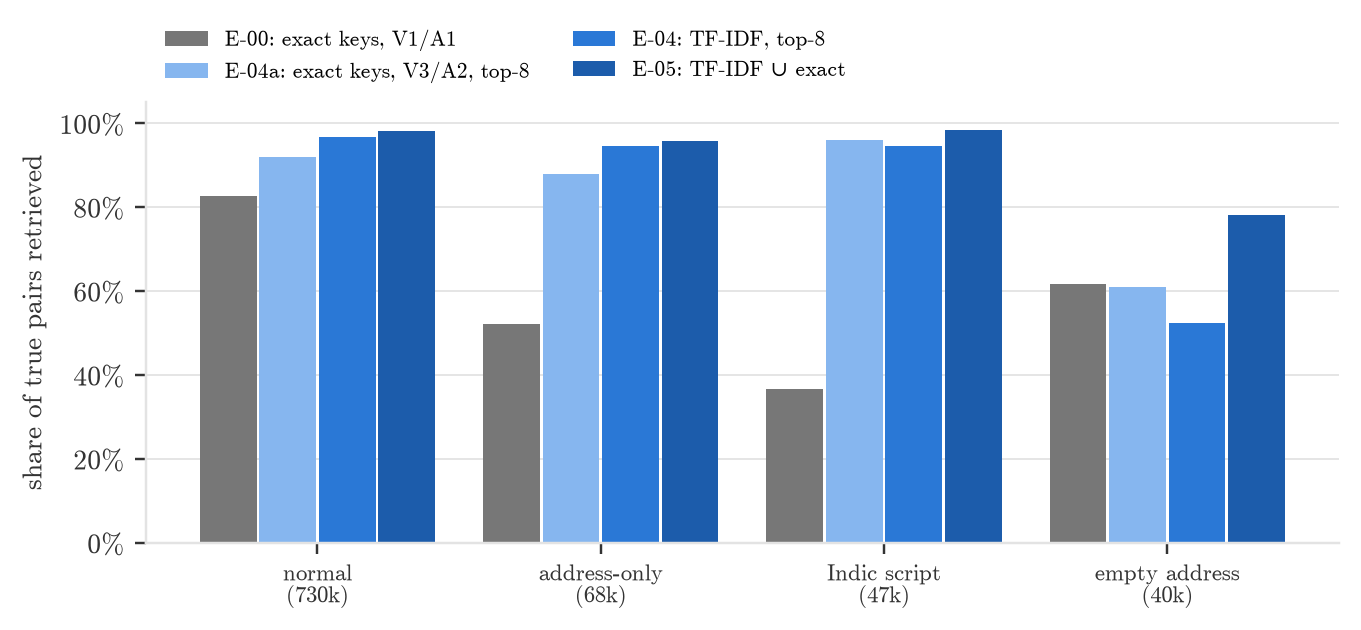
\includegraphics[width=\linewidth]{recall.png}
\caption{Share of true pairs retrieved, by type of positive (DEV-VAL). Counts are true pairs of each type.}
\label{fig:recall}
\end{figure}

\begin{table}[htbp]
\centering\small
\caption{Retrieval trade-offs on DEV-VAL. The uncapped number-set configuration exceeded the memory budget and was replaced by the top-8 cap.}
\label{tab:retrieval}
\begin{tabular}{@{}lrrrr@{}}
\toprule
Configuration & Recall & Oracle $\Fh$ & Candidates/S1 & Peak RAM \\
\midrule
E-00: exact keys, basic views & 0.770 & 0.898 & 33.0 & 3.7 GB \\
E-02: all-number set, uncapped & 0.897 & 0.958 & 117.5 & 8.2 GB \\
E-04a: all views, exact top-8 & 0.906 & 0.964 & 23.5 & 5.6 GB \\
E-04: TF-IDF top-8 & 0.945 & 0.979 & 36.0 & 5.0 GB \\
E-05: TF-IDF $\cup$ exact & \textbf{0.971} & \textbf{0.990} & 46.3 & 5.9 GB \\
\bottomrule
\end{tabular}
\end{table}

\section{Matching Model}
\label{sec:model}
\paragraph{Stage 1: pairwise evidence.} A LightGBM binary classifier (127 leaves, 400 rounds, learning rate 0.05, feature and bagging fraction 0.8) over 35 features in seven groups (Table~\ref{tab:features}). No country feature is used, because France is unseen.

\begin{table}[htbp]
\centering\small
\caption{Stage-1 feature groups.}
\label{tab:features}
\begin{tabularx}{\linewidth}{@{}lX@{}}
\toprule
Group & Features \\
\midrule
Name & token Jaccard, token intersection, token counts, token-set ratio, Levenshtein ratio, S1 name-key collisions \\
Address & token Jaccard, street Jaccard, street token-set ratio, empty-address flag, token counts \\
House number & numbers in S1 and record, cover (eq.~\ref{eq:jacc}), missing and extra numbers, first-number equality, $\Delta$ (eq.~\ref{eq:delta}), truncation \\
Legal form & relation of legal-form sets (same, dropped, added, subset, superset, changed); tokens added, dropped; \emph{Group} added \\
Out-of-vocabulary & share of name tokens used by no S1 in the block \\
Retrieval & TF-IDF score and rank, exact-key hits \\
Context & candidates per record and per S1; score, name and address gap to the record's best candidate \\
\bottomrule
\end{tabularx}
\end{table}

The legal-form and out-of-vocabulary groups came from error analysis of the first model. Among candidates with identical names and matching numbers, a record that \emph{adds} the token \emph{Group} to the S1 legal form was a true match in 0 of 837 cases. Among candidates with dissimilar names (Jaccard $< 0.2$) but similar addresses (Jaccard $\ge 0.5$), a record whose name is more than 99\% out of vocabulary was a true match in 54.6\% of cases, against 0.6\% when every name token is known: a rebrand, not a different business. The two groups raised macro $\Fh$ from 0.9605 to 0.9699.

\paragraph{Stage 2: entity-level evidence.} Pairs are not independent: a record competes for several S1s, and each S1 is supported by several records. Stage~2 keeps pairs with stage-1 probability $p_1 \ge 0.01$ (8\% of pairs, 99.94\% of retrieved positives) and adds ten features computed from other pairs' stage-1 scores:
\begin{equation}
p_2(r,e) = g\Bigl(\mathbf{x}(r,e),\; p_1(r,e),\; p_1(r,e) - \max_{e'\ne e} p_1(r,e'),\; \max_{r'\in\operatorname{sib}(r)} p_1(r',e),\; \sum_{r''\in\bar s(r)} p_1(r'',e)\Bigr),
\label{eq:stage2}
\end{equation}
where $\operatorname{sib}(r)$ are records of the same source with an identical address signature---how the per-source shared address shows up---and $\bar s(r)$ are records of the other source pointing at the same S1. Stage~2 trains on out-of-fold stage-1 scores, so it never sees scores fitted to its own labels.

\paragraph{Negatives.} Stage 1 is trained on the natural candidate distribution: every retrieved non-matching pair is a negative. 98.7\% of these 12.6M negatives receive an out-of-fold score below 0.01 and contribute almost no gradient; the 60k that score $\ge 0.1$ are the near-miss decoys and same-name collisions. Re-weighting them fivefold (E-08) left macro $\Fh$ unchanged to four decimals both before and after stage 2: the second stage already extracts what the hard negatives contain. Figure~\ref{fig:importance} shows that stage~2 is dominated by the margin to the best rival S1, a quantity no pairwise model can compute.

\begin{figure}[htbp]
\centering
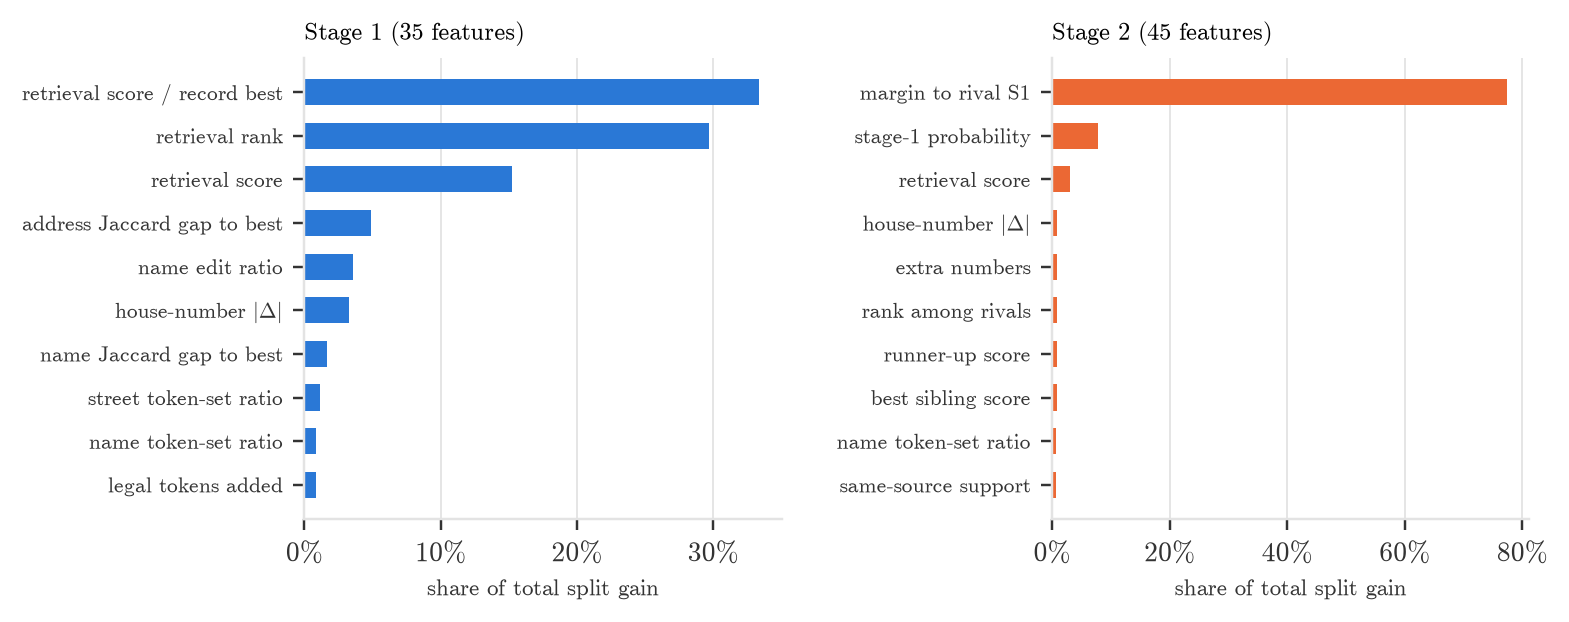
\includegraphics[width=\linewidth]{importance.png}
\caption{Share of total split gain per feature, top ten per stage.}
\label{fig:importance}
\end{figure}

\section{Decision and Assignment}
Each record is assigned to at most one S1:
\begin{equation}
a(r) = \begin{cases} \arg\max_e p_2(r,e) & \text{if } \max_e p_2(r,e) \ge \tau, \\ \emptyset & \text{otherwise,} \end{cases} \qquad \tau^* = \arg\max_\tau \text{Score}_{\text{OOF}}(\tau).
\label{eq:assign}
\end{equation}
The threshold is chosen on out-of-fold scores of the training subset, never on validation labels ($\tau^* = 0.65$). A record scored in several state blocks keeps its best S1 overall; a record without a state abstains unless its best block wins by a margin:
\begin{equation}
a(r) = \emptyset \quad \text{if} \quad p_2^{(1)}(r) - p_2^{(2)}(r) < 0.1 \text{ across blocks.}
\label{eq:margin}
\end{equation}
\paragraph{Why a global threshold near 0.65 is close to optimal.} Consider one S1 entity whose accepted list has $k$ records with calibrated probabilities $p_1\ge\dots\ge p_k$, $S=\sum_{i\le k}p_i$, and let $T=\sum_{\text{all candidates}}p_i$ estimate the number of true matches. With $\mathbb{E}[\Fh]\approx 1.25\,S/(0.25\,T+k)$, appending the next candidate $p_{k+1}$ raises the expectation iff
\begin{equation}
p_{k+1} > \frac{S}{0.25\,T+k} = 0.8\;\mathbb{E}[\Fh]_k .
\label{eq:marginal}
\end{equation}
So the right acceptance threshold is not a constant but $0.8$ times the entity's current expected score. For entities whose accepted prefix already scores $0.80$--$0.90$, which is where almost all the mass sits, eq.~\ref{eq:marginal} accepts exactly when $p > 0.64$--$0.72$. The globally tuned $\tau^*=0.65$ lies inside that band, which is why the explicit per-entity rule (E-12) recovered only $+0.0004$ over the global threshold: the constant is already the right one for the bulk of entities. Macro $\Fh$ is flat between $\tau = 0.55$ and $0.75$ (Figure~\ref{fig:tau}), so the result is not sensitive to the exact value. Three more elaborate decision rules were tested and rejected: a top-1 minus top-2 margin ($-0.0001$), a per-S1 expected-$\Fh$ prefix rule ($+0.0004$, and it lowered singleton $\Fh$ from 0.920 to 0.884), and isotonic calibration ($+0.0001$). Stage~2 already performs the entity-level reasoning these rules attempt.

\begin{figure}[htbp]
\centering
\begin{minipage}[t]{0.49\linewidth}\centering
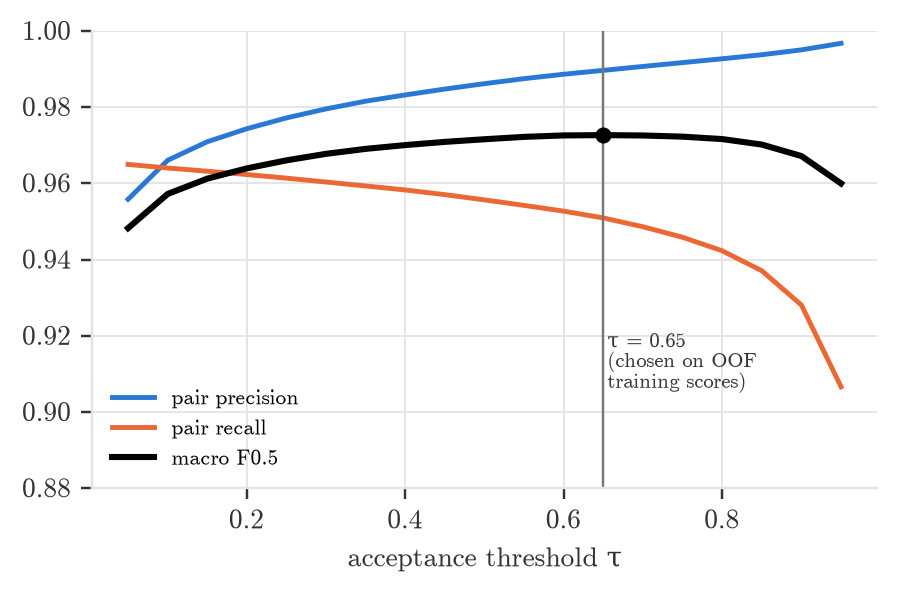
\includegraphics[width=\linewidth]{tau.png}
\end{minipage}\hfill
\begin{minipage}[t]{0.49\linewidth}\centering
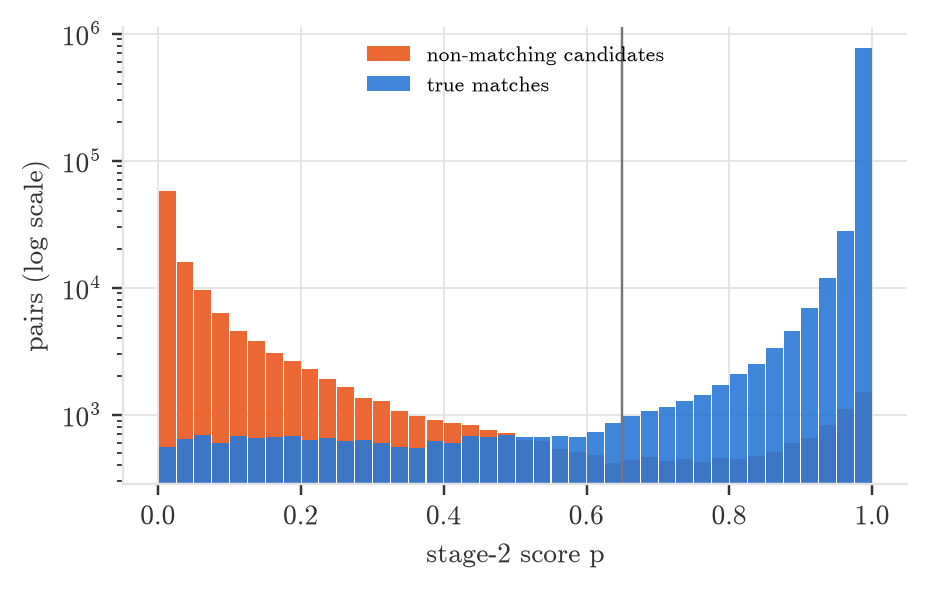
\includegraphics[width=\linewidth]{hist.png}
\end{minipage}
\caption{Left: precision, recall and macro $\Fh$ against $\tau$ (DEV-VAL). Right: stage-2 score distribution for true matches and other candidates, log scale; the vertical line marks $\tau = 0.65$.}
\label{fig:tau}
\end{figure}

\section{Experimental Method}
\label{sec:method}
\paragraph{Validation by whole states.} Decoys and same-name S1 collisions live in the same city. A random split of S1 entities would move a decoy's target to another split and make the decoy trivially rejectable. The training data was therefore split into two disjoint groups of whole US and Indian states: DEV-TRAIN (271k S1) for fitting and DEV-VAL (256k S1) for evaluation. Each subset holds all its S1s, all records they own, and all unmatched records routed to its states. DEV-VAL matches the full data closely: 5.6\% singletons (5.6\% overall), 26\% distractors (27\%), 4.68 records per S1 (4.67).

\paragraph{Admission rule.} Before any experiment ran, a written specification fixed the rule: a component is kept only if it raises DEV-VAL macro $\Fh$ by at least $+0.002$, does not hurt the cross-country transfer check, and fits the compute budget (at most 6\,GB and 15 minutes per development experiment). Each experiment changes one thing relative to its parent.

\subsection{Ablation}
\label{sec:ablation}
Figure~\ref{fig:ablation} and Table~\ref{tab:ablation} give the full record. Bootstrap 95\% intervals over S1 entities (1,000 resamples) are $[0.9695, 0.9704]$ for E-07b and $[0.9723, 0.9731]$ for E-11; they are disjoint, so the stage-2 gain is not resampling noise.

\begin{figure}[htbp]
\centering
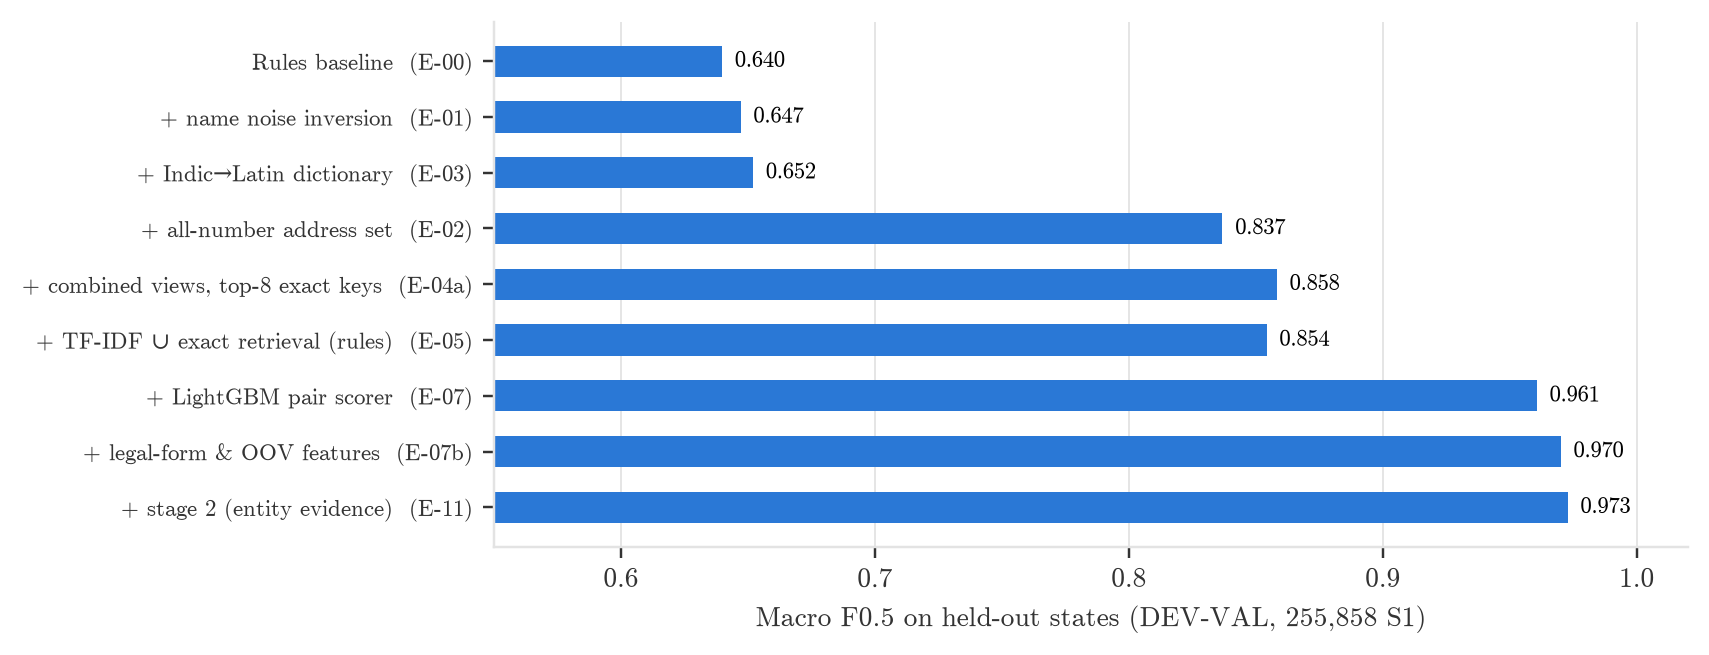
\includegraphics[width=\linewidth]{ablation.png}
\caption{Macro $\Fh$ on DEV-VAL as components were admitted; each bar adds one change to the one above.}
\label{fig:ablation}
\end{figure}

\begin{table}[htbp]
\centering\small
\caption{Complete ablation record. The three stage-2 parts were admitted together because each alone falls below the threshold; the deviation is recorded in the log.}
\label{tab:ablation}
\begin{tabular}{@{}llrrl@{}}
\toprule
ID & Change & Macro $\Fh$ & $\Delta$ & Verdict \\
\midrule
E-00 & rules baseline & 0.6397 & & baseline \\
E-01 & name noise inversion & 0.6470 & $+0.0073$ & keep \\
E-02 & all-number address set & 0.8367 & $+0.1970$ & keep \\
E-03 & Indic$\to$Latin dictionary & 0.6519 & $+0.0049$ & keep \\
E-04a & combined views, exact top-8 & 0.8581 & & reference \\
E-04 & TF-IDF retrieval (rules scorer) & 0.8495 & recall $+3.9$ pt & keep \\
E-05 & TF-IDF $\cup$ exact keys & 0.8541 & recall $+2.6$ pt & keep \\
E-07 & LightGBM stage 1 & 0.9605 & $+0.1064$ & keep \\
E-09 & top-1 minus top-2 margin & 0.9604 & $-0.0001$ & reject \\
E-12 & per-S1 expected-$\Fh$ rule & 0.9609 & $+0.0004$ & reject \\
E-13 & isotonic calibration & 0.9607 & $+0.0001$ & reject \\
E-07b & legal-form and OOV features & 0.9699 & $+0.0094$ & keep \\
E-10a & stage 2: competition & 0.9714 & $+0.0015$ & part of stage 2 \\
E-10 & $+$ siblings & 0.9721 & $+0.0007$ & part of stage 2 \\
E-11 & $+$ cross-source support & \textbf{0.9727} & $+0.0027$ (stage 2) & keep \\
E-11p & rule-based candidate pruning & 0.9712 & $-0.0015$, $3.3\times$ fewer & keep \\
E-11q & $+$ cap 50 candidates per S1 & \textbf{0.9710} & $-0.0001$ & \textbf{final} \\
E-08 & hard-negative weighting ($\times5$, OOF $p\ge0.1$) & 0.9699 & $+0.0000$ & reject \\
E-11h & stage 2 on E-08 & 0.9727 & $+0.0000$ & reject \\
E-04b & posting cap 300 & & $3\times$ join volume & reject (memory) \\
E-05c & name 5-gram retrieval (empty address) & recall 0.976 & name-only $+9.2$ pt & gate passed \\
E-07c & $+$ 5-gram candidates and features & 0.9707 & $+0.0008$ & reject (7.2 GB) \\
E-06 & dense multilingual retrieval & & $\le 1\%$ headroom & not run \\
\bottomrule
\end{tabular}
\end{table}

\section{Results at Full Scale}
The frozen configuration was run exactly as on the test set, on the full training data, and scored on the 1.94M training S1 entities outside the DEV-TRAIN states; none of them was used for fitting or threshold selection (Table~\ref{tab:full}).

\begin{table}[htbp]
\centering\small
\caption{Held-out results at development scale and at full scale.}
\label{tab:full}
\begin{tabular}{@{}lcc@{}}
\toprule
Metric & DEV-VAL (256k S1) & Full scale (1.94M S1) \\
\midrule
Macro $\Fh$ & 0.9727 & \textbf{0.9612} \\
95\% interval & $[0.9723, 0.9731]$ & $[0.9610, 0.9614]$ \\
US / India & 0.9740 / 0.9695 & 0.9705 / 0.9473 \\
Singletons & 0.9649 & 0.9516 \\
Pair precision / recall & 0.9897 / 0.9509 & 0.9847 / 0.9314 \\
Candidate recall & 0.9701 & 0.9680 \\
Oracle $\Fh$ & 0.9896 & 0.9885 \\
Candidates per S1 & 3.9 (stage 2) & 57.0 \\
\bottomrule
\end{tabular}
\end{table}

\begin{figure}[htbp]
\centering
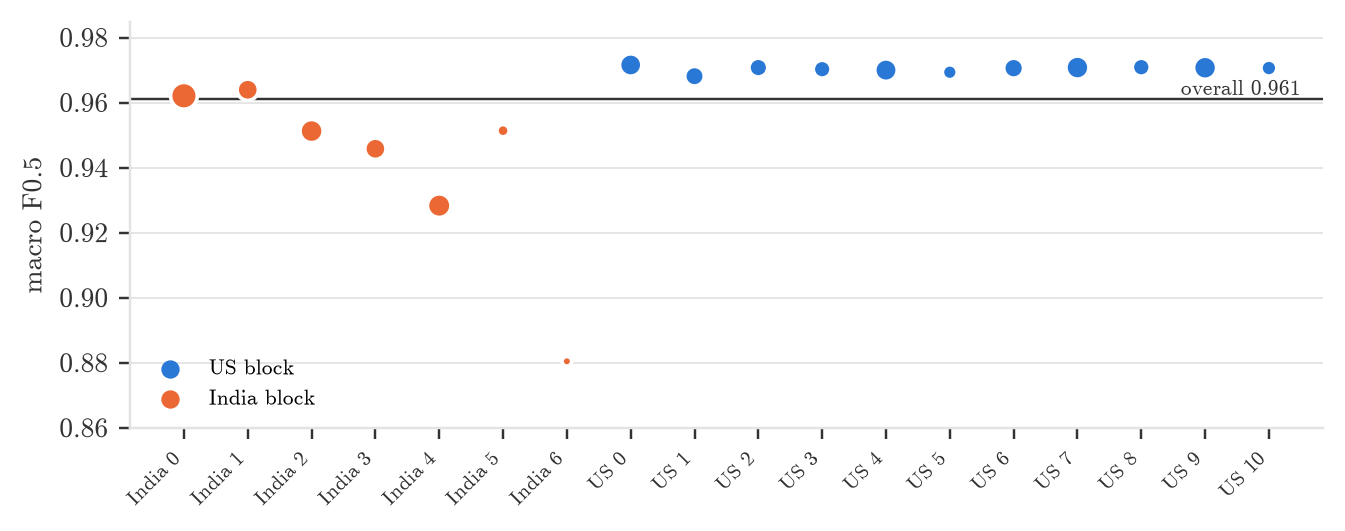
\includegraphics[width=\linewidth]{blocks.png}
\caption{Macro $\Fh$ per state block at full scale; marker area is proportional to the number of S1. US blocks are uniform (0.968--0.972); India varies with state (0.928--0.964).}
\label{fig:blocks}
\end{figure}

\paragraph{Why full scale is lower.} The first full-scale run scored 0.956. Two causes were found and fixed. (i) 13.8k Indian S1s had state names the parser did not recognise; they sat in a block their records never reached and scored 0.37. They now receive a state from the learned component map or are scored in every block of their country. (ii) Records without a state compete with same-name S1s in \emph{every} state at full scale, but only with their owner's states in the development subsets; the cross-block margin rule (eq.~\ref{eq:margin}) recovered $+0.0025$. The remaining gap of 0.011 is the cost of full-scale competition, and 0.961 is our realistic estimate of test performance.

\paragraph{Test-set behaviour.} The test predictions reproduce the structure of the training labels in all three countries, including France, for which no labels exist (Figure~\ref{fig:kdist}): 5.4--6.7\% of S1 predicted with no match against 5.6\% in training, and a mode of three matches per S1. Entities with exactly one true match are the hardest (Figure~\ref{fig:fbyk}), because one miss or one wrong merge moves their score the most.

\begin{figure}[htbp]
\centering
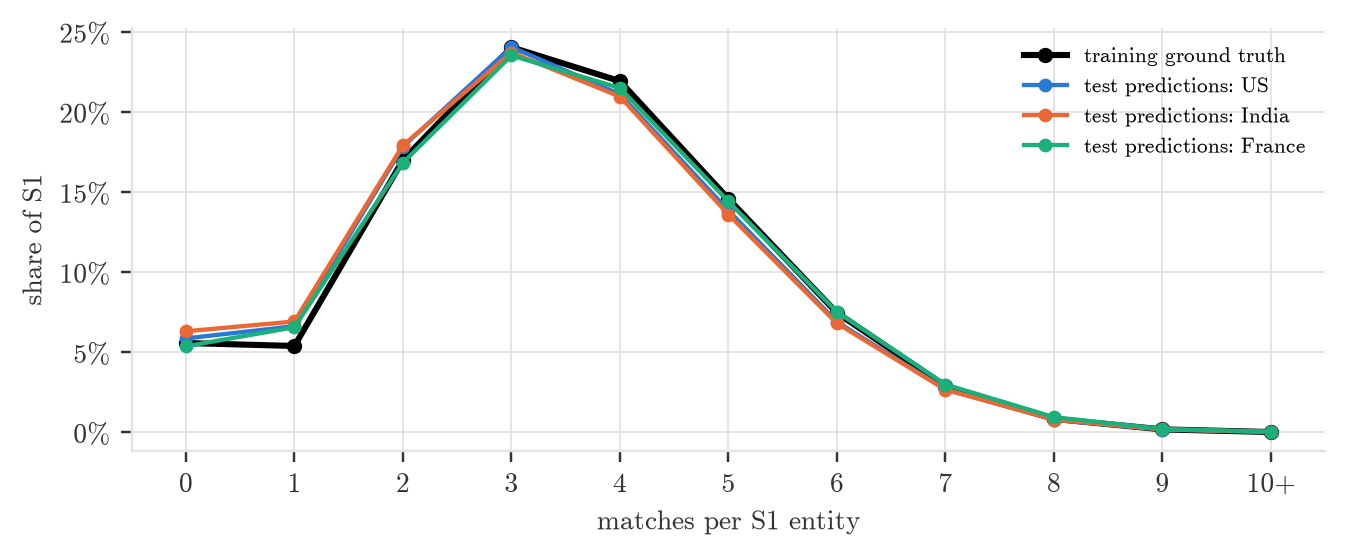
\includegraphics[width=\linewidth]{kdist.png}
\caption{Matches per S1: training ground truth against test predictions per country.}
\label{fig:kdist}
\end{figure}

\begin{figure}[htbp]
\centering
\begin{minipage}[t]{0.49\linewidth}\centering
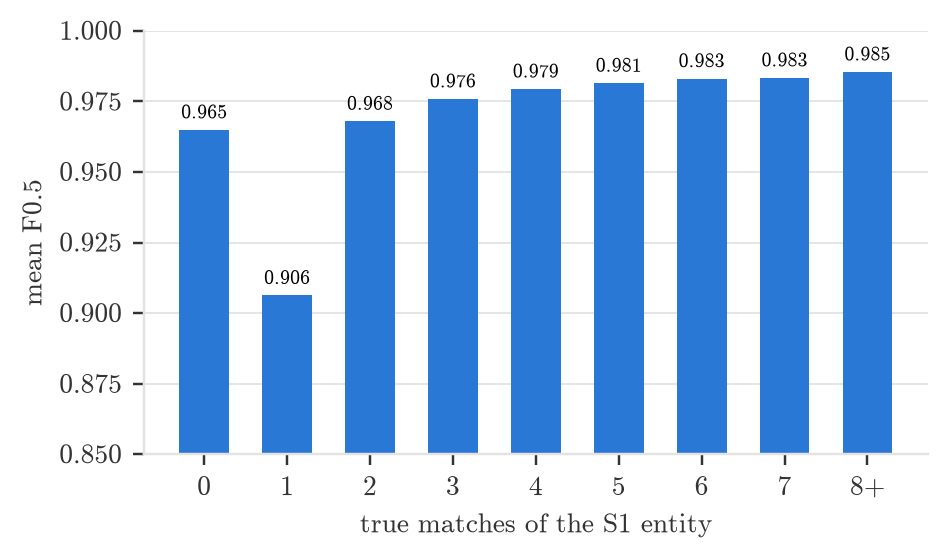
\includegraphics[width=\linewidth]{fbyk.png}
\end{minipage}\hfill
\begin{minipage}[t]{0.49\linewidth}\centering
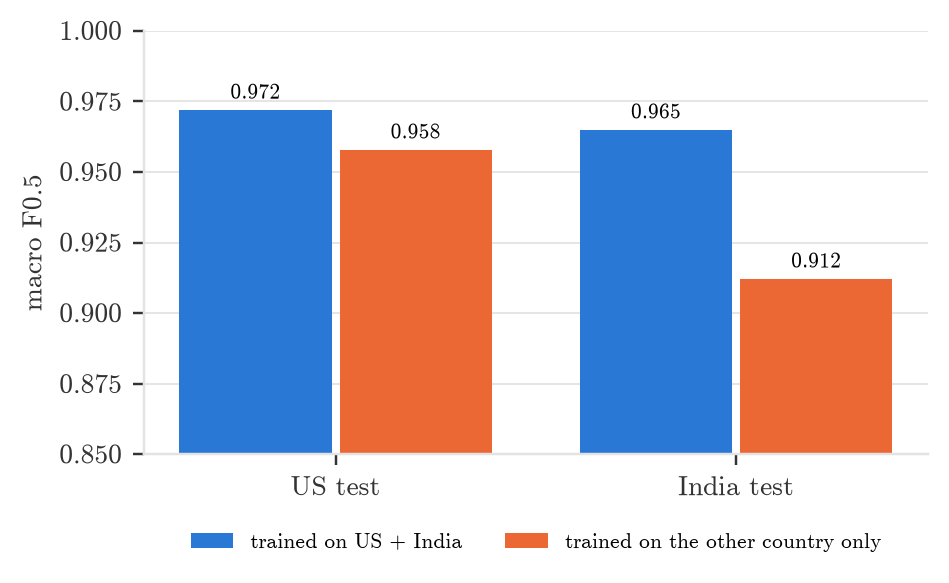
\includegraphics[width=\linewidth]{transfer.png}
\end{minipage}
\caption{Left: mean $\Fh$ by number of true matches (DEV-VAL). Right: transfer between countries (Section~\ref{sec:france}).}
\label{fig:fbyk}
\end{figure}

\section{Error Anatomy}
\label{sec:anatomy}
On DEV-VAL the final model leaves a loss of $\sum_e(1-\Fh(e)) = 6,996$ over 255,858 entities (mean $0.027$). 213,167 entities (83.3\%) are scored perfectly and 2,126 (0.8\%) score zero. Singletons account for only 505 of the loss: 505 of 14,407 singletons (3.5\%) receive a prediction. Figure~\ref{fig:anatomy} decomposes the two error types.

\begin{figure}[htbp]
\centering
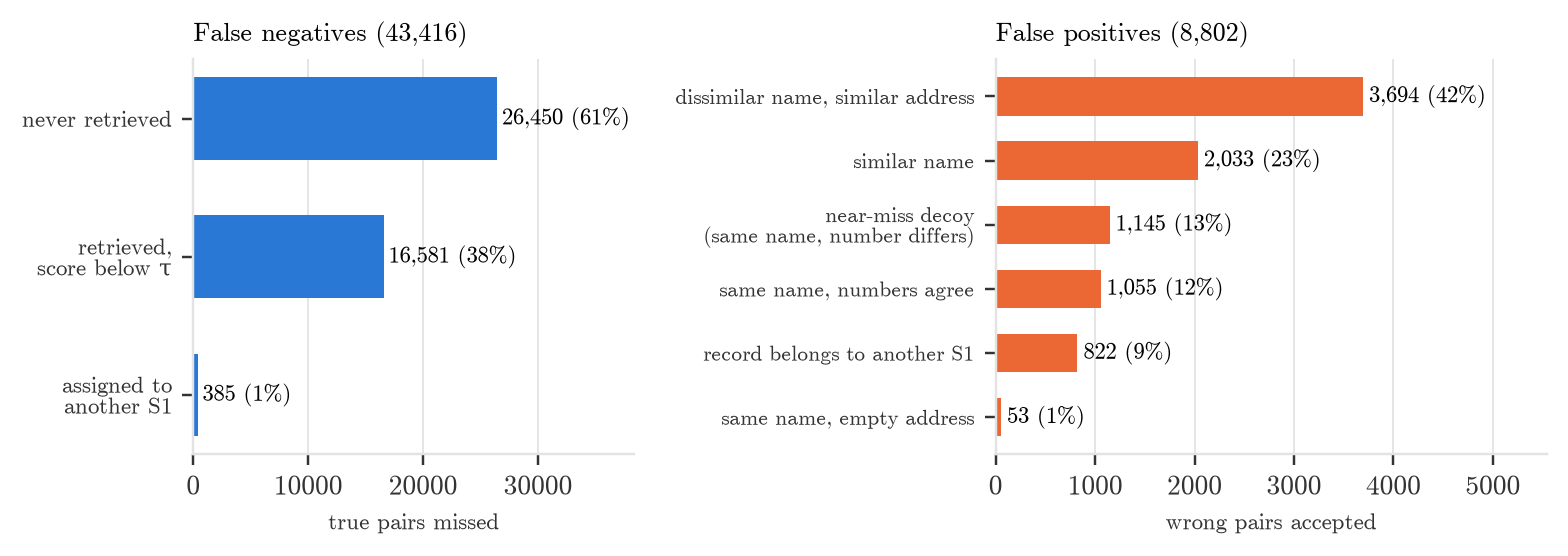
\includegraphics[width=\linewidth]{anatomy.png}
\caption{Where the remaining errors come from (DEV-VAL, final model). Left: false negatives by pipeline stage. Right: false positives by relation between the accepted record and the S1.}
\label{fig:anatomy}
\end{figure}

\paragraph{False negatives are a retrieval problem.} 26,450 of the 43,416 missed pairs (61\%) were never proposed as candidates; only 16,581 were retrieved and rejected by the scorer, and 385 were given to a rival S1. By stratum, misses are concentrated where the name carries no information: 13,629 of 40,013 empty-address positives (34.1\%) and 5,768 of 67,556 address-only positives (8.5\%) are missed, against 21,417 of 730,178 normal positives (2.9\%). The character 5-gram retriever recovered a third of the empty-address misses at the candidate stage, but the scorer could not accept them without address evidence (E-07c), so the loss here is structural: a record with an empty address and a common name is genuinely ambiguous.

\paragraph{False positives are no longer the decoys.} The near-miss decoys that dominate the raw data (Figure~\ref{fig:house}) are now 13\% of false positives (1,145 pairs); the house-number features and stage 2 have removed most of them. The largest remaining class, 42\% (3,694 pairs), is a record with a \emph{dissimilar} name at a \emph{similar} address: the out-of-vocabulary feature admits genuine rebrands, and the price is co-located businesses whose names the model cannot tell apart. The second class, ``similar name'' (23\%), is the same-name-different-street collisions inside a city. Both are precision losses that only better name evidence, not better address evidence, could reduce.

\section{Generalisation to an Unseen Country}
\label{sec:france}
France makes up 15\% of the test set and has no labels. We estimate the transfer penalty by training on one labelled country and testing on the other (Figure~\ref{fig:fbyk}, right). The penalty is small from India to the US ($-0.014$) and larger from the US to India ($-0.053$), because India carries phenomena the US lacks: native scripts, injected number prefixes and free-form addresses. France is Latin-script with structured street addresses, closer to the US case, so we expect a penalty between these values. The design limits the exposure: there is no country feature, every normalisation rule except the Indic dictionary is script- and language-agnostic, and French legal forms (SARL, SAS, SASU, EURL, SCI, SA, SNC) are handled as legal forms.

\section{Related Work}
Probabilistic record linkage goes back to Fellegi and Sunter~\cite{fellegi}, who showed that the optimal linkage rule thresholds a likelihood ratio over field agreements; our stage 1 is a learned, non-linear version of that rule, and eq.~\ref{eq:marginal} is the analogous optimal threshold for a macro list metric. Blocking as a recall/cost trade-off is surveyed by Papadakis et al.~\cite{papadakis}; our typed-token index with a document-frequency cap is a standard token-blocking scheme, and the measured cost model above is what the survey recommends reporting. Feature-based learned matchers such as Magellan~\cite{magellan} and neural matchers such as DeepMatcher~\cite{deepmatcher} and Ditto~\cite{ditto} are the two dominant families; we chose the former because the decisive signal here (the house-number relation) is a structured comparison that a string encoder must rediscover from characters, and because a 70M-pair cross-encoder pass does not fit a laptop. What is not standard is the second stage: treating a record's rival candidates, its same-source siblings and the other source as features of the pair, which converts a pairwise classifier into an entity-level one without graph propagation. LightGBM~\cite{lightgbm} is used for both stages.

\section{Compute and Reproducibility}
All runs used a 12-core laptop with 16\,GB RAM and no GPU (Table~\ref{tab:compute}). Every experiment appends one row to \texttt{experiments/experiments.csv} with its hypothesis, parent, metrics, confidence interval, runtime, peak memory and verdict. The pipeline reruns from the raw files with six commands. Only MIT, BSD or Apache-licensed libraries are used (polars, numpy, scipy, scikit-learn, rapidfuzz, LightGBM); no pretrained model, external dataset or lookup service is used.

\begin{table}[htbp]
\centering\small
\caption{Measured cost of each stage.}
\label{tab:compute}
\begin{tabular}{@{}llrr@{}}
\toprule
Stage & Scale & Time & Peak memory \\
\midrule
Ingest TSV $\to$ Parquet & 24M records & 6 s & $<2$ GB \\
Model training (both stages) & 13.6M training pairs & 2.7 min & 6.3 GB \\
Scoring one state block & $\approx$150k S1, $\approx$0.9M records & 1.5--3 min & $\le 7$ GB \\
Full test inference & 13 blocks, 38.5M candidate pairs & $\approx$20 min & $\le 7$ GB \\
Output writing & 1.73M rows, streamed by block & $<1$ min & $<4$ GB \\
\bottomrule
\end{tabular}
\end{table}

\section{Limitations}
Stated plainly, in decreasing order of expected impact.
\begin{enumerate}
\item \textbf{France is unvalidated.} French street abbreviations (R.\ for Rue, Av.\ for Avenue, Bd for Boulevard, N\textsuperscript{o}, Bis and Ter) are not normalised; a map learned without labels from test-set co-occurrence is the obvious next step.
\item \textbf{Retrieval-bound misses.} 61\% of false negatives were never retrieved, concentrated on empty-address and address-only records. A character 5-gram name retriever was tested on the weakest stratum (empty-address records): it lifts their candidate recall from 78\% to 87\% but the end-to-end gain is only $+0.0008$, because the scorer cannot separate the extra candidates without address evidence. The remaining recall lever is therefore the scorer, not retrieval (oracle $\Fh$ 0.988 at full scale).
\item \textbf{Irreducible confusions.} True matches with a genuine house-number typo ($306\to308$) are indistinguishable from decoys; $\Fh$ correctly prefers rejecting them.
\item \textbf{Threshold transfer.} $\tau$ was selected on development-scale scores. The flat curve around $\tau^*$ limits the risk, but block-scale calibration was not re-run.
\item \textbf{Deviation from the admission rule.} The three stage-2 feature groups were admitted jointly although each alone fell below $+0.002$.
\end{enumerate}

\section{Conclusion}
The largest gains came from understanding how the data was generated, not from model capacity. Comparing the set of house numbers instead of the first number was worth $+0.197$ on its own, and features modelling the decoy and rebrand operators added the precision that $\Fh$ rewards. A second stage that reasons over competing S1s, sibling records and the other source turns pairwise scores into entity-level decisions. A pre-registered admission rule kept the system small---eight components admitted, seven rejected---and the result is macro $\Fh = 0.961$ on 1.94M unseen entities at full scale, from a pipeline that scores the whole test set in about 25 minutes on a laptop.

\appendix
\section{Experiment Log}
\label{app:log}
Every run on DEV-VAL and at full scale, generated directly from \texttt{experiments/experiments.csv}. Identical reruns reproduce identical metrics; the latest row of each is shown.

\begin{center}\small
\begin{tabular}{@{}llrrrrrl@{}}
\toprule
ID & Subset & Macro $\Fh$ & Recall & Oracle & Cand./S1 & RAM (GB) & Verdict \\
\midrule
E-00 & devval & 0.6397 & 0.770 & 0.898 & 33.0 & 3.7 & INFO \\
E-00 & devtrain & 0.6388 & 0.770 & 0.898 & 40.1 & 3.9 & INFO \\
E-01 & devval & 0.6470 & 0.792 & 0.910 & 33.7 & 3.7 & KEEP \\
E-02 & devval & 0.8367 & 0.897 & 0.958 & 117.5 & 8.2 & KEEP \\
E-03 & devval & 0.6519 & 0.824 & 0.932 & 34.9 & 3.7 & KEEP \\
E-04a & devval & 0.8581 & 0.906 & 0.964 & 23.5 & 5.6 & KEEP \\
E-03x & devval & -- & -- & -- & -- & 0.0 & KILL \\
E-04 & devval & 0.8495 & 0.945 & 0.979 & 36.0 & 5.0 & KEEP \\
E-05 & devval & 0.8541 & 0.971 & 0.990 & 46.3 & 5.9 & KEEP \\
E-04b & devval & -- & -- & -- & -- & 0.0 & KILL \\
E-07 & devval & 0.9605 & 0.971 & 0.990 & 46.3 & 5.7 & KEEP \\
E-09 & devval & 0.9604 & 0.971 & 0.990 & 46.3 & 4.7 & KILL \\
E-12 & devval & 0.9609 & 0.971 & 0.990 & 46.3 & 4.7 & KILL \\
E-13 & devval & 0.9607 & 0.971 & 0.990 & 46.3 & 5.2 & KILL \\
E-07b & devval & 0.9699 & 0.971 & 0.990 & 46.3 & 6.2 & KEEP \\
E-10a & devval & 0.9714 & 0.970 & 0.990 & 3.9 & 4.3 & INFO \\
E-10 & devval & 0.9721 & 0.970 & 0.990 & 3.9 & 4.3 & INFO \\
E-11 & devval & 0.9727 & 0.970 & 0.990 & 3.9 & 4.3 & KEEP \\
E-14 & devval & -- & -- & -- & -- & 9.1 & INFO \\
G3-full & train\_full & 0.9560 & 0.963 & 0.985 & 56.7 & 4.0 & INFO \\
G3-full & train\_full & 0.9612 & 0.968 & 0.988 & 57.0 & 4.2 & KEEP \\
E-05c & devval & 0.8541 & 0.976 & 0.991 & 46.7 & 4.9 & INFO \\
E-07c & devval & 0.9707 & 0.976 & 0.991 & 46.7 & 7.0 & KILL \\
E-08 & devval & 0.9699 & 0.971 & 0.990 & 46.3 & 9.3 & KILL \\
E-11h & devval & 0.9727 & 0.970 & 0.989 & 3.9 & 4.4 & KILL \\
E-07p & devval & 0.9687 & 0.968 & 0.988 & 14.0 & 2.9 & INFO \\
E-11p & devval & 0.9712 & 0.967 & 0.988 & 3.8 & 2.4 & KEEP \\
E-07q & devval & 0.9687 & 0.967 & 0.988 & 13.6 & 3.1 & INFO \\
E-11q & devval & 0.9710 & 0.966 & 0.988 & 3.8 & 2.5 & KEEP \\
\bottomrule
\end{tabular}
\end{center}

\section{Notation}
\begin{center}\small
\begin{tabular}{@{}ll@{}}
\toprule
Symbol & Meaning \\
\midrule
$e$, $r$ & an S1 entity; an S2/S3 record \\
$M_e$, $\hat M_e$ & true and predicted match sets of $e$ \\
$\N(\cdot)$ & set of numbers in an address, leading zeros removed \\
$N_c$, $\mathrm{df}_t$ & S1 entities in block $c$; S1 entities containing token $t$ \\
$p_1$, $p_2$ & stage-1 and stage-2 match probabilities \\
$\tau$ & acceptance threshold ($\tau^* = 0.65$) \\
$\operatorname{sib}(r)$, $\bar s(r)$ & same-source siblings of $r$; records of the other source \\
\bottomrule
\end{tabular}
\end{center}


\begin{thebibliography}{9}\small
\bibitem{fellegi} I.~P. Fellegi and A.~B. Sunter. A theory for record linkage. \emph{Journal of the American Statistical Association}, 64(328):1183--1210, 1969.
\bibitem{papadakis} G. Papadakis, D. Skoutas, E. Thanos, and T. Palpanas. Blocking and filtering techniques for entity resolution: a survey. \emph{ACM Computing Surveys}, 53(2), 2020.
\bibitem{magellan} P. Konda et al. Magellan: toward building entity matching management systems. \emph{PVLDB}, 9(12):1197--1208, 2016.
\bibitem{deepmatcher} S. Mudgal et al. Deep learning for entity matching: a design space exploration. \emph{SIGMOD}, 2018.
\bibitem{ditto} Y. Li, J. Li, Y. Suhara, A. Doan, and W.-C. Tan. Deep entity matching with pre-trained language models. \emph{PVLDB}, 14(1):50--60, 2020.
\bibitem{lightgbm} G. Ke et al. LightGBM: a highly efficient gradient boosting decision tree. \emph{NeurIPS}, 2017.
\end{thebibliography}

\end{document}
